\documentclass[mythesis.tex]{subfiles}
\begin{document}
% tells latex when compiling a subfile what chapter number this document is
% set the chapter to minus one as \chapter will increment the counter
\setcounter{chapter}{1}
\chapter{Relativistic Wave Equations and a lot of other stuff}

\section{The Bethe-Salpeter Equation}

It is useful to introduce a simple model for the introduction of the ideas
and formalism of the Bethe-Salpeter equation. For this purpose, consider
a simple field theory of two heavy scalar particles interacting by the
exchange of a light scalar particle. This model allows  consideration of the
basic structure of the Bethe-Salpeter equation without dealing with the
complication of spin and the exchange of multiple mesons as is necessary
in a realistic model of the deuteron. The equations
resulting from this simple analysis will be extended to include these
complications in Section VI.

The Bethe-Salpeter equation \cite{BetheSalpeter} for a two-body system
can be derived from
quantum field theory and a rigorous derivation is outlined in Refs.
\cite{Lurie,CoesterandRiska}.
Here,  simple arguments are used to suggest the form and content of the
Bethe-Salpeter equation. First, consider all of the Feynman diagrams that
contribute for the scattering of two heavy scalars, which can be thought
of as scalar nucleons, by the exchange of a
light scalar meson as represented in Fig. \ref{scat1}.
%
\begin{figure}
\centerline{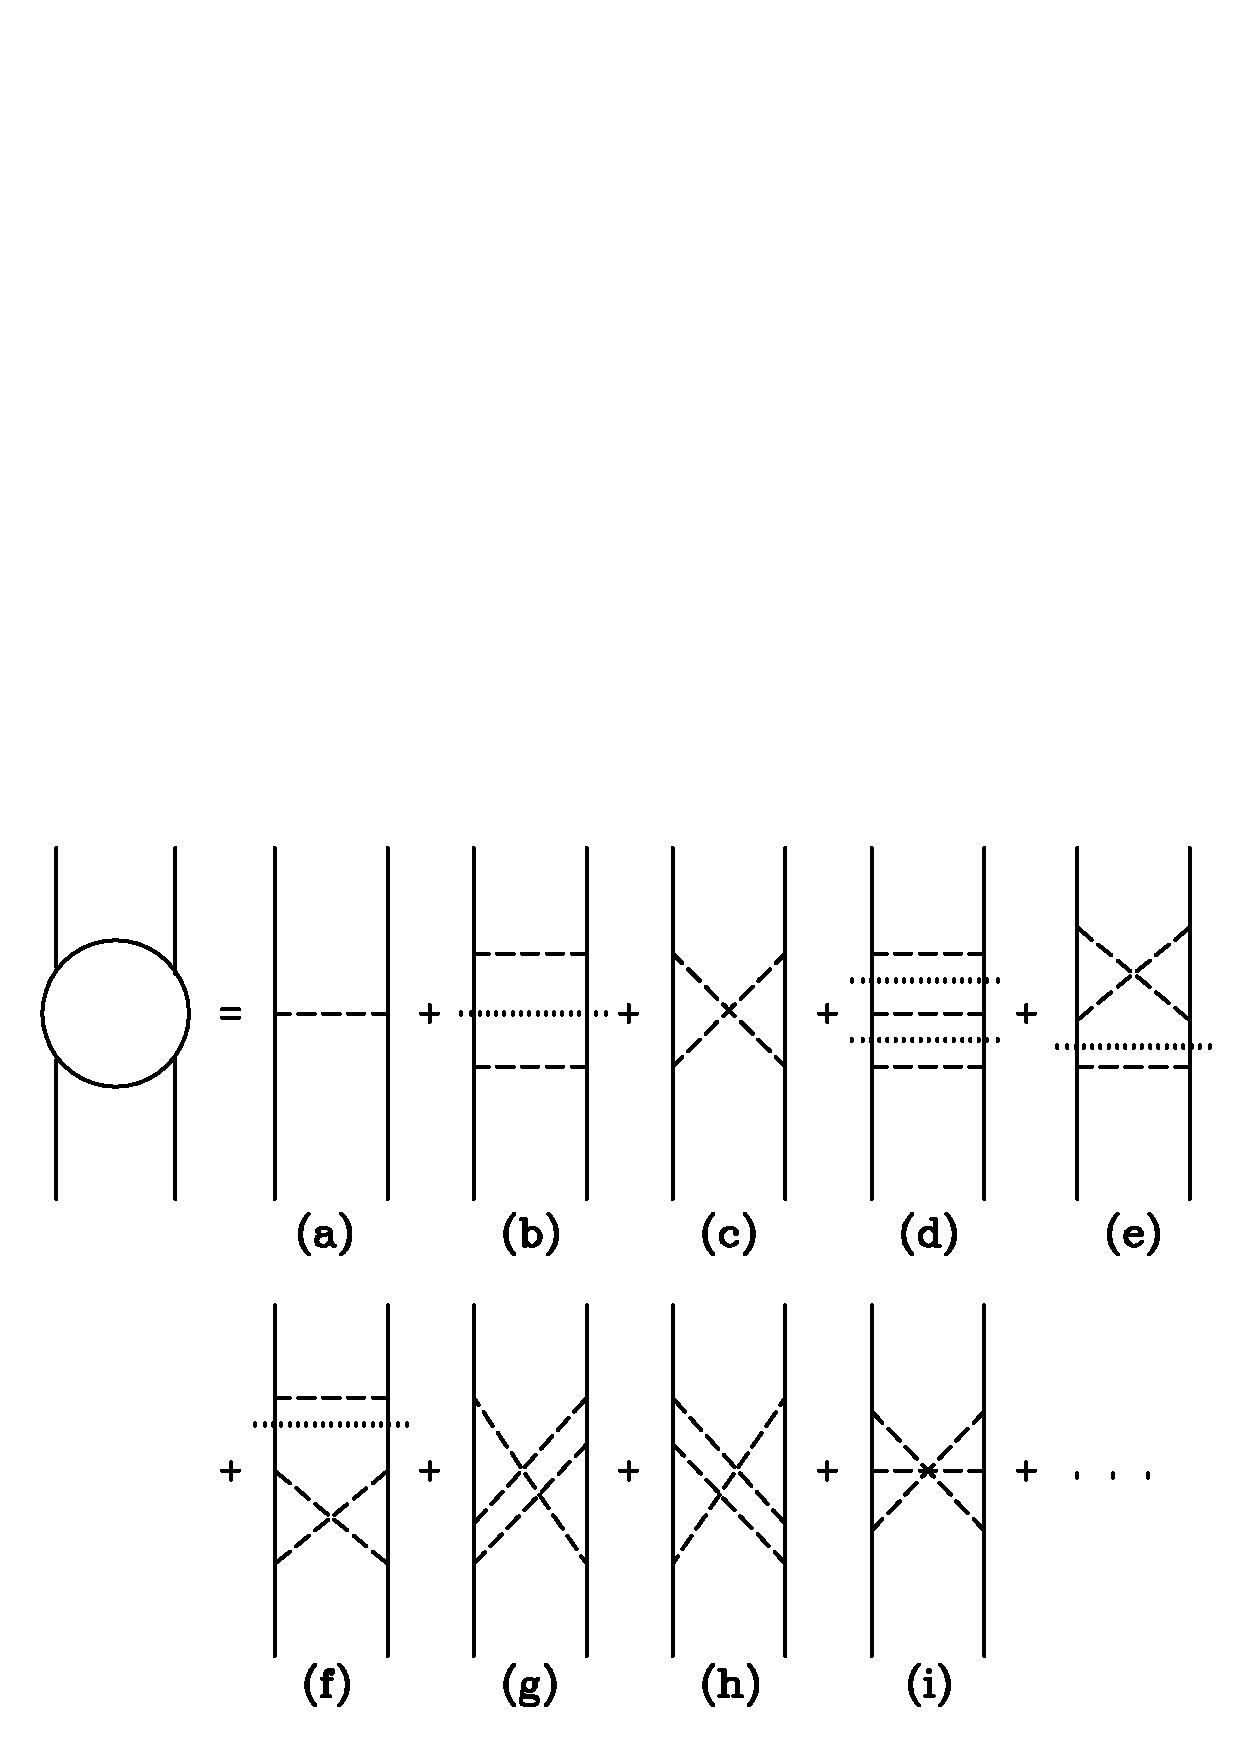
\includegraphics[width=4in]{graphics/new/scat1.pdf}}
\vspace*{12pt} \caption{Feynman diagrams representing the
scattering of two heavy scalar nucleons (solid lines) by the
exchange of a light scalar mesons (dashed lines. Dotted lines show
two-nucleon cuts for reducing the diagrams.} \label{scat1}
\end{figure}
%
The solid lines
represent propagators for the scalar nucleons and the dashed lines
represent propagators for the scalar mesons.
These diagrams are
intended to represent skeleton diagrams where all diagrams which represent
dressings of propagators or three point vertices are subsumed into the
propagators or vertices. Diagrams (\ref{scat1}b) and (\ref{scat1}d) are
double and triple
iterations of diagram (\ref{scat1}a). Diagrams (\ref{scat1}e) and
(\ref{scat1}f) are diagram (\ref{scat1}c) preceded
and followed by diagram (\ref{scat1}a). This suggests a scheme for summing
all of the
contributions to the scattering matrix. This is done by introducing the
concept of a two-particle irreducible diagram. A diagram which can not be
separated into two or more diagrams by cutting just two nucleon propagators
is said to be irreducible. By this definition, the diagrams (\ref{scat1}b),
(\ref{scat1}d), (\ref{scat1}e)
and (\ref{scat1}f) are reducible since they can be cut into two or more
simple diagrams
as illustrated by the dotted lines in Fig. \ref{scat1}.
The remaining diagrams, (\ref{scat1}a), (\ref{scat1}c),
(\ref{scat1}g), (\ref{scat1}h) and (\ref{scat1}i) are irreducible since
any cut across the diagrams will
cut at least one meson propagator as well as the two nucleon propagators.

\begin{figure}
\centerline{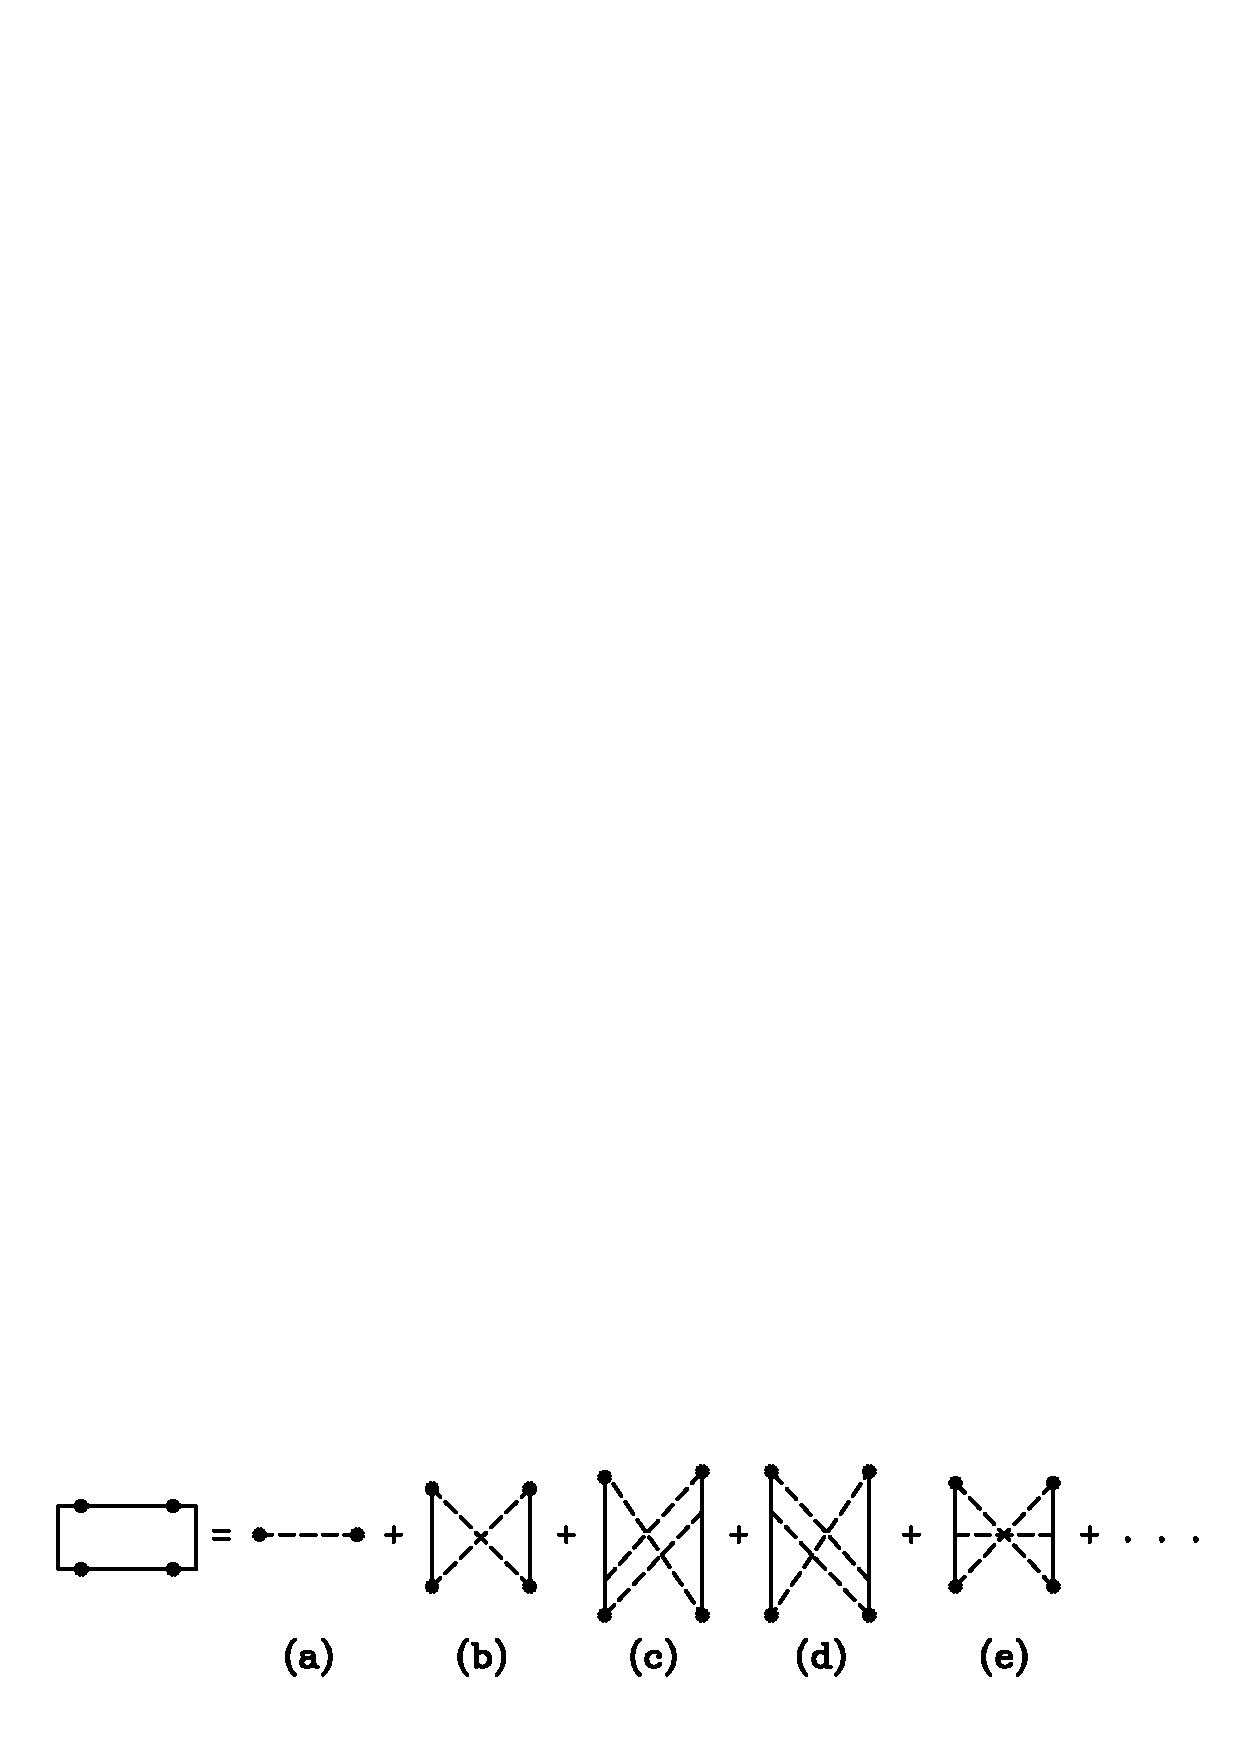
\includegraphics[width=5.5in]{graphics/new/kernel.pdf}}
\caption{Feynman diagrams representing the two-nucleon irreducible
kernel.} \label{reduce}
\end{figure}

If the Bethe-Salpeter interaction kernel $V$ is defined to be the sum of
all two-particle irreducible diagrams as represented by the diagrams in
Fig. \ref{reduce}, the sum of all possible contributions
to the $\cal M$ matrix can be represented diagramatically by Fig.
\ref{BStmatrix}.
%
\begin{figure}
\centerline{\includegraphics[width=3in]{graphics/new/bst.pdf}}
\caption{Feynman diagramatical representation of the
Bethe-Salpeter equation for the $\cal M$ matrix.}\label{BStmatrix}
\end{figure}
%
This equation treats the nucleon degrees of freedom explicitly while all of
the meson degrees of freedom are contained in the interaction kernel.
Standard Feynman rules can be used to obtain an integral equation for the
$\cal M$ matrix. This can be represented as
%
\begin{equation}
{\cal M}(p',p;P)=V(p',p;P)-\int\frac{d^4k}{(2\pi)^4} V(p',k;P) G_0(k;P)
{\cal M}(k,p;P),\label{BSt}
\end{equation}
%
or equivalently,
%
\begin{equation}
{\cal M}(p',p;P)=V(p',p;P)-\int\frac{d^4k}{(2\pi)^4} {\cal M}(p',k;P)
G_0(k;P) V(k,p,;P),\label{BStA}
\end{equation}
%
where $P$ is the total four-momentum of the nucleon pair, and $p'$, $k$ and
$p$
are the final, intermediate and initial relative four-momenta of the
nucleon pair. The two-nucleon intermediate propagator is defined as
%
\begin{equation}
G_0(k;P)=-i \Delta^{(1)}_F(\frac{P}{2}+k,m) \Delta^{(2)}_F(\frac{P}{2}-k,m),
\end{equation}
%
where
%
\begin{equation}
\Delta^{(i)}_F(p,m)=\frac{1}{p^2-m^2+i\eta}
\end{equation}
%
is the propagator for particle $i$ with mass $m$. Note only
the pole part of the  dressed single-particle progagator is retained, as is
conventional in such models. The contributions from the residual part of the
propagator can be included in a variety of ways, but this complication
is ignored here.

The equations for the conjugate of the $\cal M$ matrix
%
\begin{equation}
{\cal M}^\dagger (p',p;P)=V^\dagger (p',p;P)-\int\frac{d^4k}{(2\pi)^4}
{\cal M}^\dagger (p',k;P)
G_0^\dagger(k;P) V^\dagger(k,p,;P),\label{BStC}
\end{equation}
%
and
%
\begin{equation}
{\cal M}^\dagger(p',p;P)=V^\dagger (p',p;P)-\int\frac{d^4k}{(2\pi)^4}
V^\dagger (p',k;P) G_0^\dagger (k;P)
{\cal M}^\dagger (k,p;P),\label{BStCA}
\end{equation}
%
can be used to derive the unitarity relation for the $\cal M$ matrix
%
\begin{eqnarray}
{\cal M}(p',p,;P)&-&{\cal M}^\dagger (p',p;P)= \nonumber \\
& &\int\frac{d^4k'}{(2\pi)^4}\int\frac{d^4k}{(2\pi)^4}\left( (2\pi)^4
\delta^4(p'-k')-{\cal M}^\dagger (p',k';P)G_0^\dagger(k';P)\right) \nonumber\\
& &\times\left( V(k',k;P)-V^\dagger (k',k;P)\right) \nonumber \\
& &\times\left( (2\pi)^4\delta^4(k-p)-G_0(k;P) {\cal M}(k,p;P)\right) \nonumber\\
& &-\int\frac{d^4k}{(2\pi)^4}{\cal M}^\dagger(p',k;P)
\left( G_0(k;P)-G_0^\dagger (k;P)\right) {\cal M}(k,p;P).\label{unitarity}
\end{eqnarray}
%
The discontinuity in the $\cal M$ matrix, which in this simple case is
simply the imaginary part of the amplitude,
arises from two
contributions, one involving the discontinuity of the two-nucleon free
propagator and the other involving the discontinuity of the kernel.
The discontinuity of the free two-nucleon propagator is proportional to
the product of two delta functions placing both of the nucleons on their
mass shells. This can occur only when the $P^2\geq (2m)^2$. If
the invariant mass of the pair $W$ is defined such that $P^2=W^2$, then
this can occur only when $W\geq 2m$ or $W\leq -2m$. Since the discontinuity
of the free propagator occurs within a four-momentum loop, this
produces branch cuts beginning at the two thresholds in $W$. These are
the positive and negative energy elastic cuts. The discontinuity of the
kernel is associated with both nucleons and at least one meson being on
mass shell and contributes a set of overlapping cuts with thresholds at
$W=\pm (2 m + n \mu)$, where $\mu$ is the meson mass and $n>0$ is an integer.
The analytic structure of the  $\cal M$ matrix as a function of complex
$W$ is shown in Fig. \ref{analyticM}.
%
\begin{figure}
\centerline{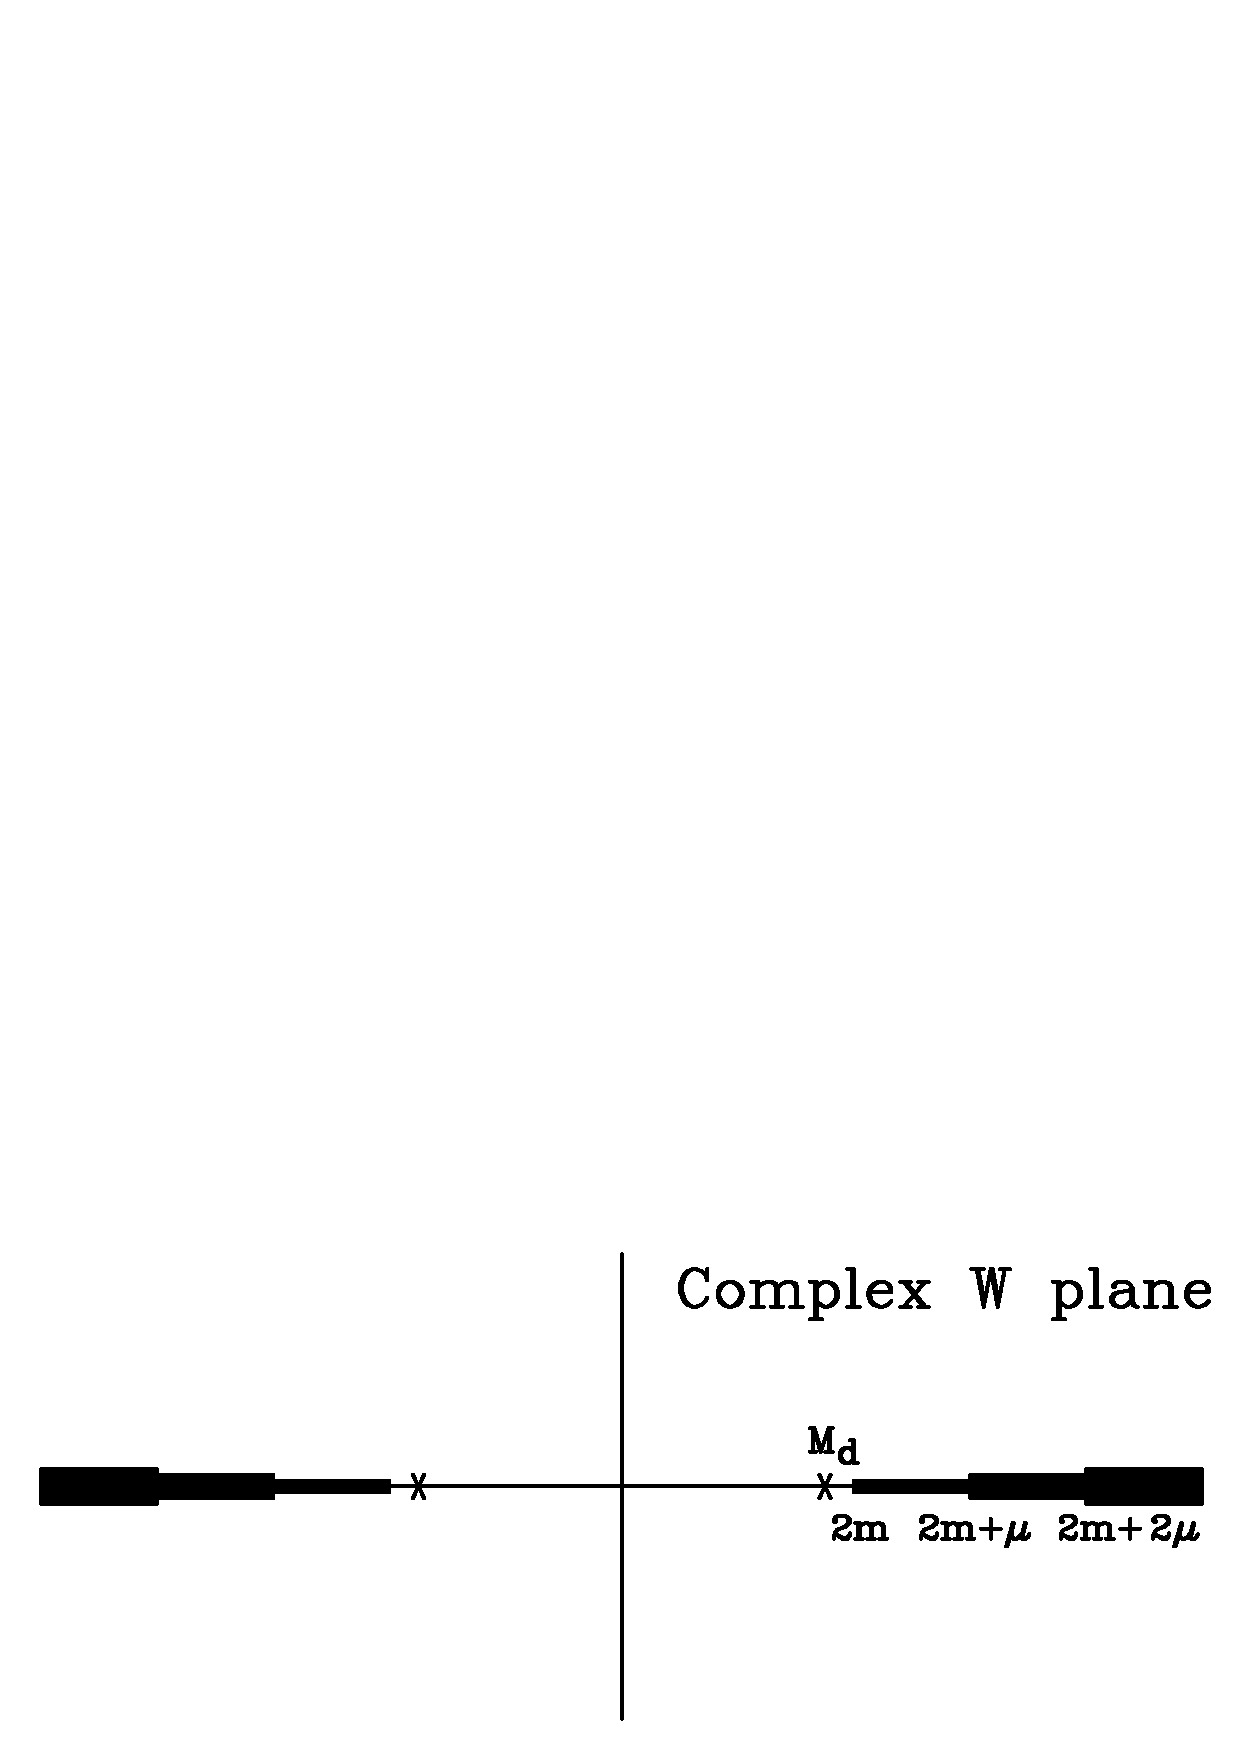
\includegraphics[width=4in]{graphics/new/analytic.pdf}}
\caption{The analytic structure of the $\cal M$ matrix as a
function of complex $W$. The heavy lines represent branch cuts and
crosses represent bound state poles.}\label{analyticM}
\end{figure}
%
Another possibility, that is obscured by writing the unitarity relation as
in (\ref{unitarity}), is that the $\cal M$ matrix can have poles
corresponding to the presence of bound states. For the purpose of
discussion, assume that there is only one bound state for
$P^2=P_d^2=M_d^2<4 m^2$, where $M_d$ is the mass of the scalar ``deuteron.''
Thus, poles are expected in $\cal M$ at $W=\pm M_d$ and are illustrated in
Fig. \ref{analyticM} by crosses.

The $\cal M$ matrix can now be represented as
%
\begin{equation}
{\cal M}(p',p,;P)=\frac{\Gamma(p';P_d)\Gamma^\dagger(p;P_d)}
{P^2-M_d^2+i\eta}+{\cal R}(p',p,;P), \label{Mpole}
\end{equation}
%
where ${\cal R}(p',p,;P)$ represents the remainder of the $\cal M$ matrix
once the pole is removed. Substituting (\ref{Mpole}) into (\ref{BSt}) gives
%
\begin{eqnarray}
& &\frac{\Gamma(p';P_d)\Gamma^\dagger(p;P_d)}
{P^2-M_d^2+i\eta}+{\cal R}(p',p,;P) =V(p',p;P)\nonumber \\
& & \qquad -\int\frac{d^4k}{(2\pi)^4} V(p',k;P) G_0(k;P)\left(
\frac{\Gamma(k;P_d)\Gamma^\dagger(p;P_d)}
{P^2-M_d^2+i\eta}+{\cal R}(k,p,;P)\right) .
\end{eqnarray}
%
Since $V$, $G_0$ and $\cal R$ are analytic at the bound state poles,
comparing the residue of the pole on each side of the equation yields
%
\begin{equation}
\Gamma(p';P_d)=-\int\frac{d^4k}{(2\pi)^4} V(p',k;P_d) G_0(k;P_d)
\Gamma(k;P_d).\label{BSvertex}
\end{equation}
%
$\Gamma(p';P_d)$ is the Bethe-Salpeter bound state vertex function. The
normalization of the bound state is obtained by first using (\ref{BSt})
and (\ref{BStA}) to obtain the nonlinear form of the Bethe-Salpeter
equation
%
\begin{eqnarray}
& &{\cal M}(p',p,;P)=V(p',p;P)-\int\frac{d^4k}{(2\pi)^4}{\cal M}(p',k;P)
G_0(k;P) {\cal M}(k,p,;P) \nonumber \\
& &\qquad -\int\frac{d^4k'}{(2\pi)^4}\int\frac{d^4k}{(2\pi)^4}
{\cal M}(p',k';P) G_0(k';P)V(k',k;P) G_0(k;P) {\cal M}(k,p,;P).\nonumber \\
\label{nonlinear}
\end{eqnarray}
%
Substituting (\ref{Mpole}) into (\ref{nonlinear}) and equating the residues
of the poles gives:
\begin{eqnarray}
1&=&\int\frac{d^4k}{(2\pi)^4}\Gamma^\dagger(k;P_d)
\left. \frac{\partial ~~}{\partial P^2}G_0(k;P)\right|_{P_d}\Gamma(k;P_d)
\nonumber\\
&-&\int\frac{d^4k'}{(2\pi)^4}\int\frac{d^4k}{(2\pi)^4}
\Gamma^\dagger(k';P_d)G_0(k';P_d)\left. \frac{\partial ~~}{\partial P^2}
V(k',k;P)\right|_{P_d} G_0(k;P_d)\Gamma(k;P_d),\nonumber \\
\end{eqnarray}
where the Bethe-Salpeter vertex equation (\ref{BSvertex}) has been used to
simplify the expression.
The Bethe-Salpeter bound state wave function can now be defined as:
\begin{equation}
\psi(p;P_d)= G_0(p;P_d)\Gamma(p;P_d)\label{BSwave}
\end{equation}
and, using the fact that $G_0(k';P_d)$ is hermitian, the wave function
normalization is given by:
\begin{eqnarray}
1&=&\int\frac{d^4k}{(2\pi)^4}\psi^\dagger(k;P_d)G^{-1}_0(k;P_d)
\left. \frac{\partial ~~}{\partial P^2}G_0(k;P)\right|_{P_d}G^{-1}_0(k;P_d)
\psi(k;P_d)
\nonumber\\
&-&\int\frac{d^4k'}{(2\pi)^4}\int\frac{d^4k}{(2\pi)^4}
\psi^\dagger(k';P_d)\left. \frac{\partial ~~}{\partial P^2}
V(k',k;P)\right|_{P_d} \psi(k;P_d) \label{normal}
\end{eqnarray}
Using the definition of the wave function (\ref{BSwave}), and the equation
for the vertex function (\ref{BSvertex}) a wave equation can be written
as
%
\begin{equation}
G^{-1}_0(p;P_d)\psi(p;P_d)=-\int\frac{d^4k}{(2\pi)^4}V(p,k;P_d)\psi(k;P_d)
\label{BSwaveEq}
\end{equation}

The basic formalism is now in place for both scattering and normalized bound
states. There are, however, substantial practical difficulties in obtaining
such solutions. Although the equations as they are presented are exact,
they can not be solved exactly since the kernel contains an infinite
number of contributions. Therefore, it is conventional to retain only a
limited number of contributions to the kernel in order to obtain a solution.
Typically, the kernel is truncated at the level of one- or two-boson
exchange. This truncation constitutes an almost inevitable approximation
and, as will be discussed below,  for the scalar
model used here, it is not the best approximation to the
full untruncated Bethe-Salpeter equation.

A second problem, that is of a technical nature, is the difficulty of
solving the four-dimensional integral equations. The equations can be reduced
to two-dimensional equations by an expansion of the potentials, scattering
matrices and vertex functions in some suitable set of angular functions.
This leaves integrals in the loop energy and the magnitude of the loop
momentum. As is usually the case with performing such loop integrations, it
is convenient to perform a Wick rotation of the energy variable into the
complex plane. Due to the presence of branch cuts associated with the
angular expansion of the kernel, which move as a function of the external
relative energy, the contour must be carefully distorted in performing
the Wick rotation. The two-dimensional integral equations can, and have
been solved numerically \cite{Tjon,Zuilhof,Umnikov}.

\section{Quasipotential Equations}

An alternate approach, to the construction of relativistic models of two-body
bound and scattering states is the construction of quasipotential equations.
This method can be understood in relation to the Bethe-Salpeter equations
presented above. The common characteristic of all quasipotential equations
is the replacement of the free two-nucleon propagator by a new propagator
that includes a delta-function constraining the relative energy of the
intermediate states and thereby reducing the four-dimensional integral
equation to three dimensions. Although it is possible to express this
replacement in completely covariant terms \cite{BrownandJ}, it is most
easily described in
the center of momentum frame where the equations are generally actually
solved. By introducing a new propagator of the form
\begin{equation}
g_0(p;P)=\frac{\pi}{E_p}\delta\left( p_0-x(E_p-W/2)\right) \hat g_0(p;P),
\label{QPprop}
\end{equation}
where $E_p=\sqrt{{\bf p}^2+m^2}$ is the on-mass-shell energy,
the multiple scattering series represented by (\ref{BSt}) can be rearranged
into a pair of coupled integral equations
\begin{equation}
{\cal M}(p',p;P)=U(p',p;P)-\int\frac{d^3k}{(2\pi)^3 2 E_k} U(p',\check k;P)
\hat g_0(\check k;P)
{\cal M}(\check k,p;P),\label{QPt}
\end{equation}
and
\begin{equation}
U(p',p;P)=V(p',p;P)-\int\frac{d^4k}{(2\pi)^4} V(p',k;P)\left( G_0(k;P)
-g_0(k;P)\right) U(k,p;P)\label{QuasiPot}
\end{equation}
where $\check k$ represents the intermediate-state relative momentum
constrained by the delta function in (\ref{QPprop}), and the new kernel
in (\ref{QPt}), defined by (\ref{QuasiPot}), is called the quasipotential.
The equations (\ref{QPt}) and (\ref{QuasiPot}) are exactly equivalent to
(\ref{BSt}). Note that while (\ref{QPt}) is a three-dimensional integral
equation, the equation for the quasipotential (\ref{QuasiPot}) is still
four-dimensional. Matters have only been complicated at this stage by
replacing one four-dimensional integral equation with a three-dimensional
plus a four-dimensional integral equation. In practice, the (\ref{QuasiPot})
is not solved exactly, but is iterated and then truncated at a fixed number
of meson exchanges. This reduces the construction of $U$ to a quadrature over loops
containing $V$. Indeed, in most cases, both the Bethe-Salpeter and
quasipotential equations are solved in one-boson exchange or ladder
approximation. In this approximation $U=V$.

The quasipotential equation for the vertex function is
%
\begin{equation}
\Gamma(p;P_d)=-\int\frac{d^3k}{(2\pi)^3 2E_k} U(p,\check k;P_d)
\hat g_0(\check k;P_d)
\Gamma(\check k;P_d)\label{QPvertex}
\end{equation}
%
Note that the vertex function on the right side of (\ref{QPvertex}) depends
only upon the constrained relative momentum while the vertex function on
the left depends upon the unconstrained momentum. The unconstrained
vertex function is, therefore, obtained in two steps. First the integral
equation is solved with only the constrained relative momentum $\check p$
appearing on the left of (\ref{QPvertex}). The resulting constrained
vertex function can then be substituted into the right side of (\ref{QPvertex})
and the unconstrained vertex function obtained by quadrature. A similar
approach can be applied to the solution of (\ref{QPt}).

A constrained quasipotential wave function can be defined as
%
\begin{equation}
\hat\psi(\check p;P_d)\equiv \hat g_0(\check p;P_d) \Gamma(\check p;P_d)
\end{equation}
%
The normalization condition for these wave functions can be obtained in a
similar fashion to that use in obtaining (\ref{normal}) and is
%
\begin{eqnarray}
1&=&\int\frac{d^3k}{(2\pi)^3 2 E_k}\hat\psi^\dagger(\check k;P_d)
\hat g^{-1}_0(\check k;P_d)
\left. \frac{\partial ~~}{\partial P^2}\hat g_0(\check k;P)
\right|_{P_d}\hat g^{-1}_0(\check k;P_d)
\hat \psi(\check k;P_d)
\nonumber\\
&-&\int\frac{d^3k'}{(2\pi)^3 2 E_{k'}}\int\frac{d^3k}{(2\pi)^3 2 E_k}
\hat \psi^\dagger(\check k';P_d)\left. \frac{\partial ~~}{\partial P^2}
U(\check k',\check k;P)\right|_{P_d} \hat \psi(\check k;P_d) \label{QPnormal}
\end{eqnarray}
%
The wave equation for the constrained quasipotential wave function is
%
\begin{equation}
\hat g^{-1}_0(\check p;P_d)\hat\psi(\check p;P_d)=
-\int\frac{d^3k}{(2\pi)^3 2 E_k}U(\check p,\check k;P)
\hat \psi(\check k;P_d)\label{QPwaveEq}
\end{equation}

Criteria for choosing $\hat g_0$ can be obtained by considering the analytic
structure of the $\cal M$ matrix as shown in Fig. \ref{analyticM}. Knowing
the analytic structure, it is possible to construct dispersion relations for
the scattering matrix. If the system is lightly bound, the physical values
of W will be close to the elastic cut on the positive energy
real W axis. The contributions to the scattering matrix coming from the
positive energy cuts and poles should then constitute the dominant
contributions to the scattering matrix. In order to preserve this property,
it is necessary to choose $\hat g_0$ such that it preserves the position
and residues associated with the positive energy elastic cut. This
requirement allows for an infinite variety of choices for $\hat g_0$ and
a substantial number of quasipotential propagators have been proposed in
the literature. A representative sample for our scalar model is presented
in Table \ref{quasitable}.
\begin{table}
\caption{A selection of quasipotential propagators for scalar nucleons}
\label{quasitable}
\vspace{12pt.}
\begin{center}
\begin{tabular}{lcc}\hline\hline
Name & x & $\hat g_0(\check p,P)$ \\
\hline
 & & \\
Blankenbecler-Sugar \cite{BSLT} & 0 & $\frac{1}{2(E^2_p-\frac{W^2}{4})-i\eta}$  \\
 & & \\
Thompson \cite{Thompson} & 0 & $\frac{1}{W(2E_p-W)-i\eta}$  \\
 & & \\
Todorov \cite{Todorov}  & 0 & $\frac{E_p}{W(E^2_p-\frac{W^2}{4})-i\eta}$ \\
 & & \\
Gross (spectator) \cite{GrossA} & 1 & $\frac{1}{W(2E_p-W)-i\eta}$  \\
 & & \\
Erkelenz-Holinde  \cite{Erkelenz} & 1 & $\frac{1}{2(E^2_p-\frac{W^2}{4})-i\eta}$  \\
 & & \\
Kadychevsky  \cite{Kadychevsky} & 1 &  $\frac{1}{2E_p(2E_p-W)-i\eta}$ \\
 & & \\
Gross  \cite{GrossB} & $-1\leq x\leq 1$ &$\frac{2E_p}{W(2E_p-W)(E_p+\frac{W}{2}+
        x^2(E_p-\frac{W}{2}))}$\\ \hline\hline
\end{tabular}
\end{center}
\end{table}
%

Before examining the results of calculations performed in the simple scalar
model, it is useful to compare the Bethe-Salpeter and quasipotential
equations. As a practical matter, both types of equations require that a
truncated kernel be used for calculating scattering amplitudes and bound
state wave functions, usually at the level of the ladder or one-boson-exchange
approximation. The question then arises as to which of these equations
provides the best approximation to the complete untruncated Bethe-Salpeter
equation, which is the exact field-theoretical result. It is tempting to
assume that the ladder approximation to the Bethe-Salpeter equation is the
optimal approximation, in that it appears the most straightforward and least
arbitrary prescription for truncating the equations. There is good reason
to believe that this is not necessarily the case. The simple scalar model
that is used here for pedagogical purposes has received a considerable
amount of study. In particular, Gross \cite{GrossBook} has examined this
model in considerable
detail and has shown that to all orders in the Feynman diagramatical
expansion of the scattering matrix there is a partial cancellation between
iterated ladder-like contributions and contributions from the crossed boxes.
The particular organization of the $\cal M$ matrix equations associated with
the spectator equation places the canceling pieces of the iterated ladders
and the crossed boxes in higher-order contributions to the quasipotential
and therefore improves the convergence of the truncated spectator equation
to the full Bethe-Salpeter equation. This can also be seen in Table VI.1
of Ref. \cite{BrownandJ} which compares the coefficients of an expansion
in $\mu/m$ of
the second order contributions to the scattering matrix for several of
the quasipotential equations and the full second order Bethe-Salpeter
result. All of the approaches agree to order $(\mu/m)^{-1}$. All of the
quasipotential approaches agree with the full second-order Bethe-Salpeter
to order $(\mu/m)^{0}$, but the ladder approximation to the Bethe-Salpeter
equation disagrees at this order. Some caution should be used in
generalizing these results to systems involving particles with spin and
isospin, in that the operators associated with these quantities can interfere
with the delicate cancellations that occur in the scalar model. In these
more complicated situations, the question of the quality of any particular
approximation is still open. Some additional light can, however, be cast on
the practical implications of this problem by some additional results from
the study of the simple scalar model under conditions which approximate
the use of these quasipotential equations in physical applications.

\subsection{This is a Subsection}

Four score and seven years ago, our forefathers brought forth on this
continent a new nation conceived in liberty and dedicated to the proposition
that all men are created equal.

\section{The Scalar Model}

It is useful to now construct a version of the scalar model that has
features that appear in the calculations of the deuteron presented
in Section VI. First, in any phenomenological model of the
deuteron that treats the effective degrees of freedom as nucleons and
mesons, information about the finite size of this constituents must be
included as form factors at the interaction vertices. The general form of
the nucleon-nucleon-meson vertex in our scalar model would be
%
\begin{equation}
-i g F(p'^2,p^2,\ell^2) \label{strongvert}
\end{equation}
%
where $g$ is a dimensionful coupling constant, $p$ and $p'$ are the initial
and final nucleon four-momenta, and $\ell=p-p'$ is the meson four-momentum.
$F(p'^2,p^2,\ell^2)$ is a general form factor depending upon the invariant
masses of the three virtual particles connecting to the interaction vertex.
For simplicity, assume that the form factor can be written in a
factorable form \cite{FVOHA,FVOHB,GrossandRiska}
%
\begin{equation}
F(p'^2,p^2,\ell^2)=h(p'^2)h(p^2)f(\ell^2)\label{factorable}
\end{equation}
%
where the meson form factor is taken to be
%
\begin{equation}
f(\ell^2)=\frac{(\Lambda_\mu^2-\mu^2)^2+\Lambda_\mu^4}
{(\Lambda_\mu^2-\ell^2)^2+\Lambda_\mu^4}
\end{equation}
%
and the nucleon form factor is
%
\begin{equation}
h(p^2)=\frac{2(\Lambda_n^2-m^2)^2}{(\Lambda_n^2-p^2)^2+(\Lambda_n^2-m^2)^2}
\end{equation}
%
where $\Lambda_\mu$ and $\Lambda_n$ are meson and nucleon form factor masses.
The presence of the nucleon form factor is an unusual feature of the
calculations presented here. This form factor allows the four-momenta of the
nucleons to be controlled such that the contributions from highly-virtual
nucleons can be limited.

Since the model is to be solved for a variety of quasipotential equations,
it is necessary to deal with an additional problem. For all quasipotential
propagators for which $x\neq 0$, the intermediate state nucleons in
(\ref{QPt}) are not treated symmetrically. This can lead to problems with
the Pauli exchange symmetry of the scattering amplitudes and vertex
functions. It has been shown in Ref. \cite{FVOHB} that this problem can be
overcome
by requiring that the interaction kernel be symmetrized for bosons or
antisymmetrized for fermions. Therefore, the kernel for the quasipotential
equations should be taken as
%
\begin{eqnarray}
V(p',p;P)&=& \frac{1}{2}g^2 h((P/2+p')^2)h((P/2-p')^2)\nonumber \\
& &\times\left[f((p-p')^2) \Delta_F(p-p',\mu)+f((p+p')^2)
\Delta_F(p+p',\mu)\right]\nonumber \\
& &\times h((P/2+p)^2)h((P/2-p)^2).
\end{eqnarray}
%
for the scalar model, where it is assumed that the exchanged meson carries
no charge.
This procedure has the drawback that it can generate spurious singularities
in the calculation of scattering amplitudes and vertex functions. This
problem can be dealt with as shown in Ref. \cite{FVOHB}.

It is useful to use a procedure in choosing the parameters in the model that
is consistent with the methods used to constrain the model parameters in
meson-nucleon models of the deuteron. Any acceptable model of the deuteron
must contain an interaction that produces the deuteron bound state
at the correct binding energy and that provides a reasonable description
of the scattering data up to a few hundred MeV of laboratory kinetic
energy. Since it is intended that this scalar model  bear some
resemblance to the
deuteron, the scalar nucleon mass is chosen to be $m=938.9~MeV$, the
meson mass to be $\mu=138.0~MeV$ and the meson form factor mass is fixed to
be $\Lambda_\mu=2500.0~MeV$, which is of the same order as the meson
form factor masses found in the fits to the deuteron and the NN scattering
data in Refs. \cite{FVOHA,FVOHB}. For each calculation, the value of
the nucleon form factor
mass is fixed, but  various values of this parameter are considered in
order to examine
the sensitivity of the calculations to this parameter.
If  the nucleon, meson and form factor masses are fixed,
the only remaining parameter in this simple scalar model is the coupling
constant. The procedure used in producing these calculations for the scalar
model is to adjust the coupling constant for each quasipotential model to
produce an S-wave bound state at a binding energy of $2.3~MeV$. This value
is then
used to calculate the S- and D-wave phase shifts for the model.

\begin{figure}
\centerline{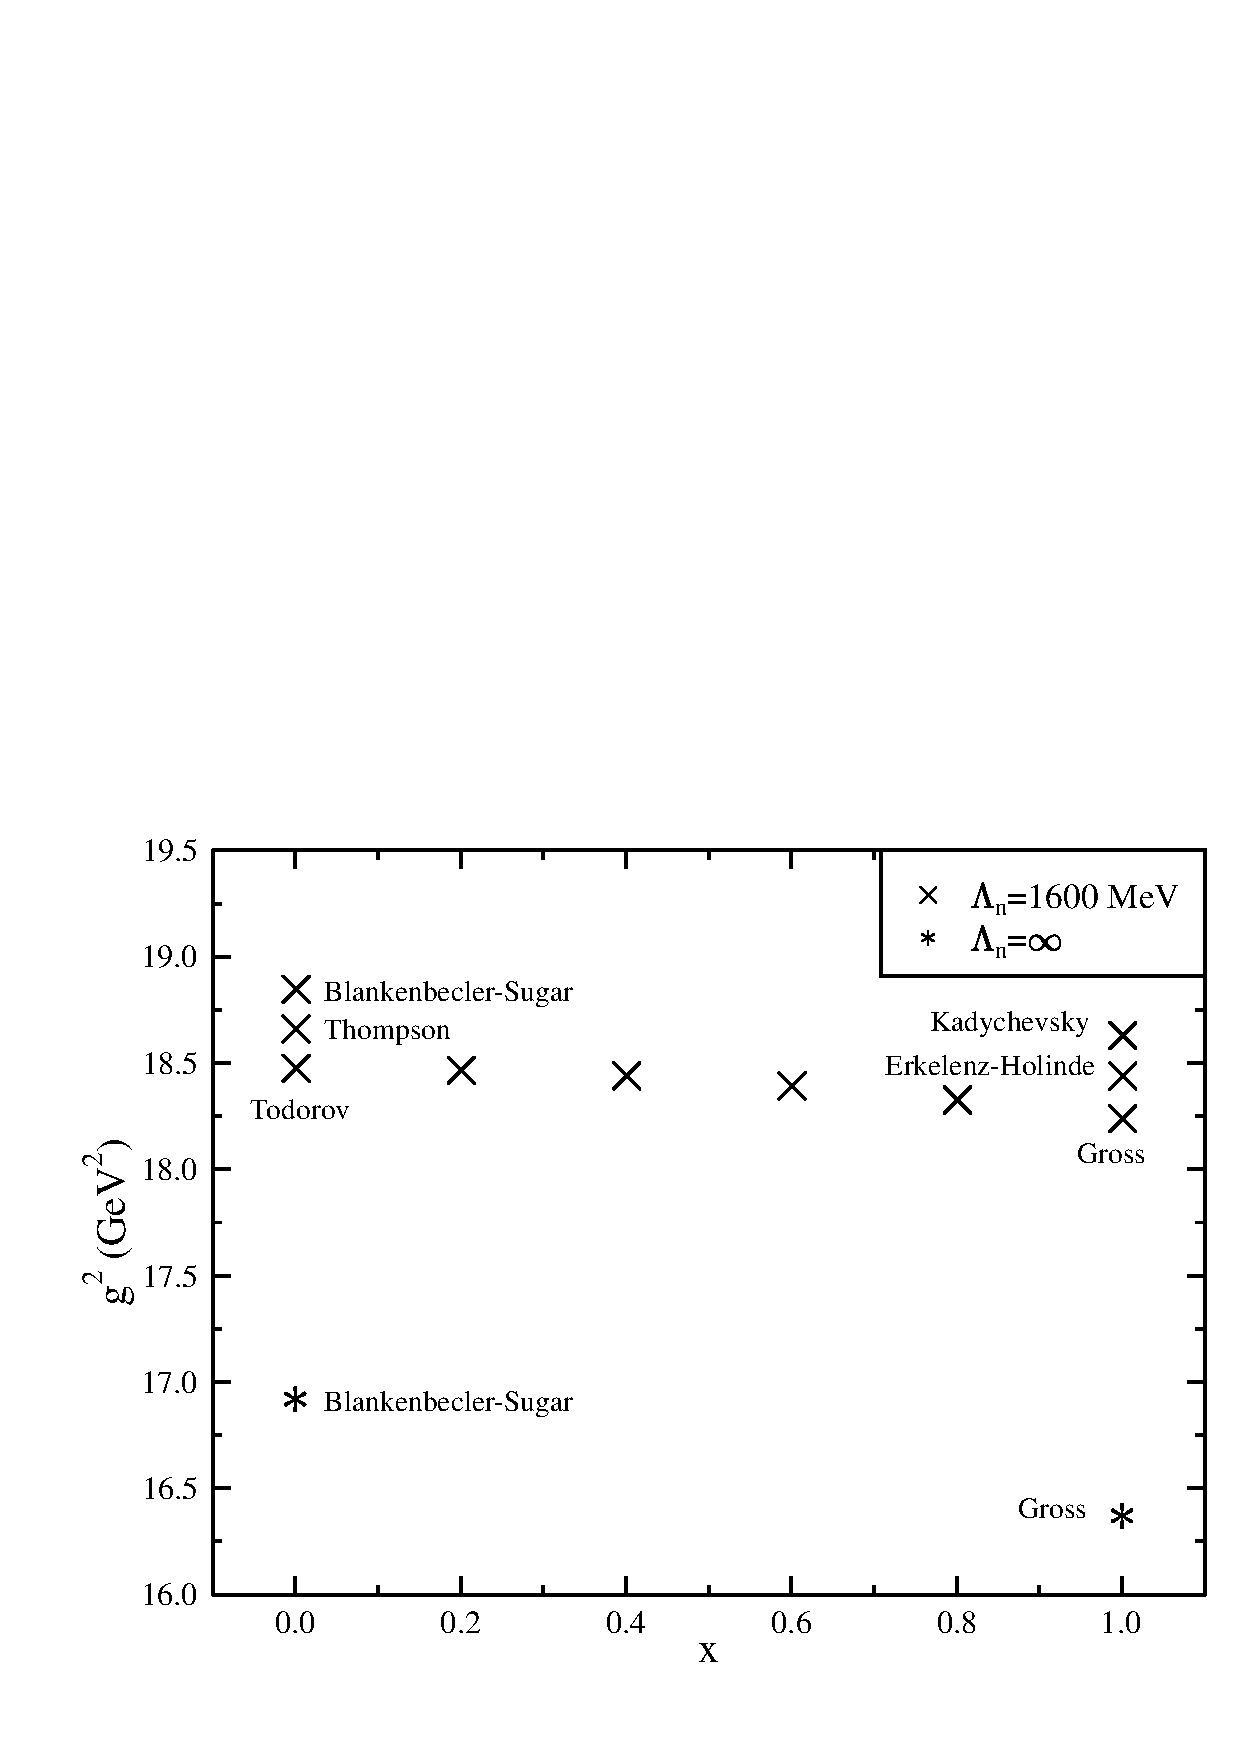
\includegraphics[width=4.5in]{graphics/coupling.pdf}}
%\vspace*{12pt}
\caption{This figure shows square of the coupling constants for the
various quasipotential
models listed in Table I. The crosses represent couplings calculated
with a nucloen form factor mass of $\Lambda_n=1600~MeV$. The asterisks
represent couplings calculated with $\Lambda_n=\infty$.}\label{couplings}
\end{figure}


Figure \ref{couplings} shows the values of the square of the coupling
constants for the various quasipotential models listed in Table I as a
function of the quasipotential parameter $x$. The
crosses are calculated with a nucleon form factor mass $\Lambda_n=1600~MeV$,
and the asterisks are calculated with $\Lambda_n=\infty$. Values for
$-1<x<1$ are for the family of quasipotential models described in
Ref. \cite{GrossB}. Clearly, the coupling constant depends both on the quasipotential
model used and the value of the nucleon cutoff. However, for a fixed cutoff
mass, the variation in the value of $g^2$ is on the order of a few percent.
In these models, the couplings should be viewed as effective coupling
constants.
%


\begin{figure}
\centerline{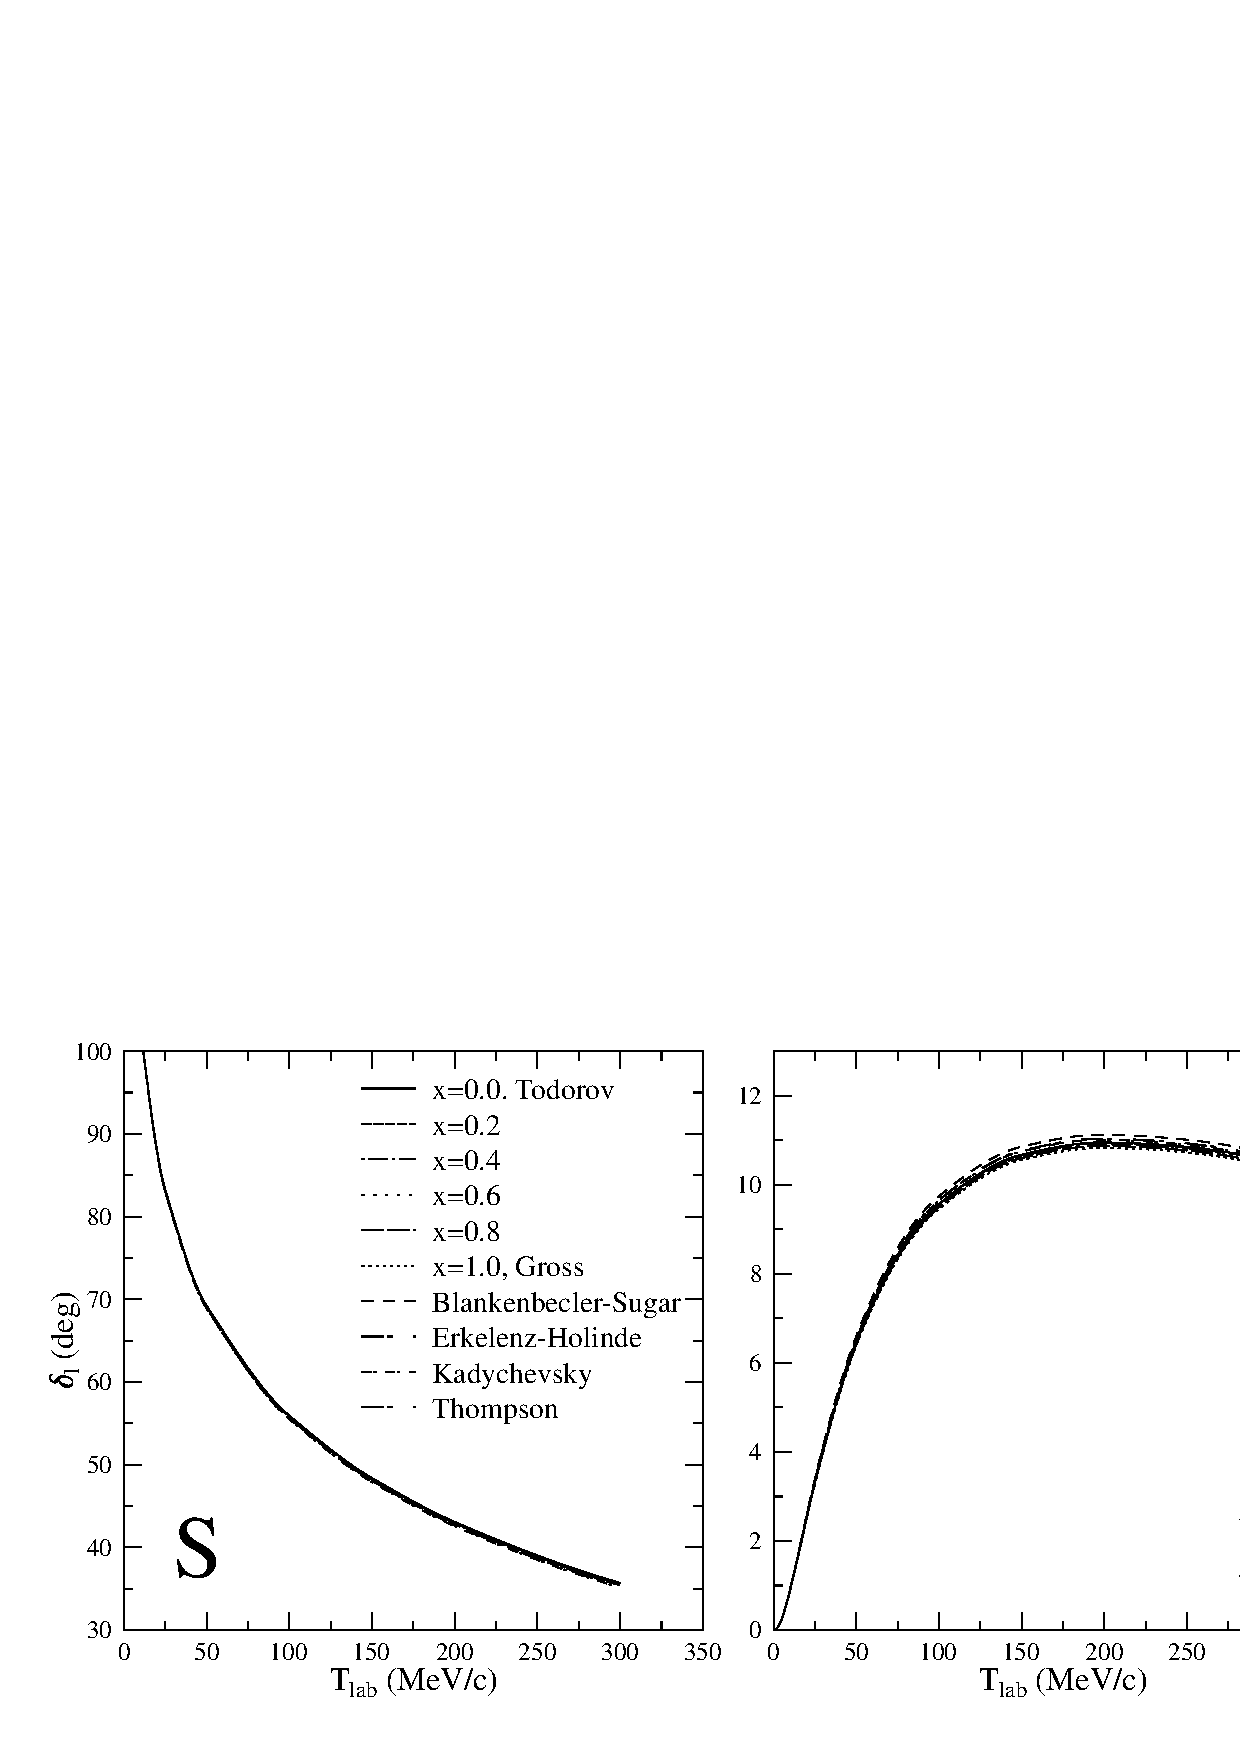
\includegraphics[width=5.5in]{graphics/phase_coup.pdf}}
\caption{S- and D- wave phase shifts calculated for the various
models listed in Table I with
$\Lambda_n=1600~MeV$.}\label{QPphases}
\centerline{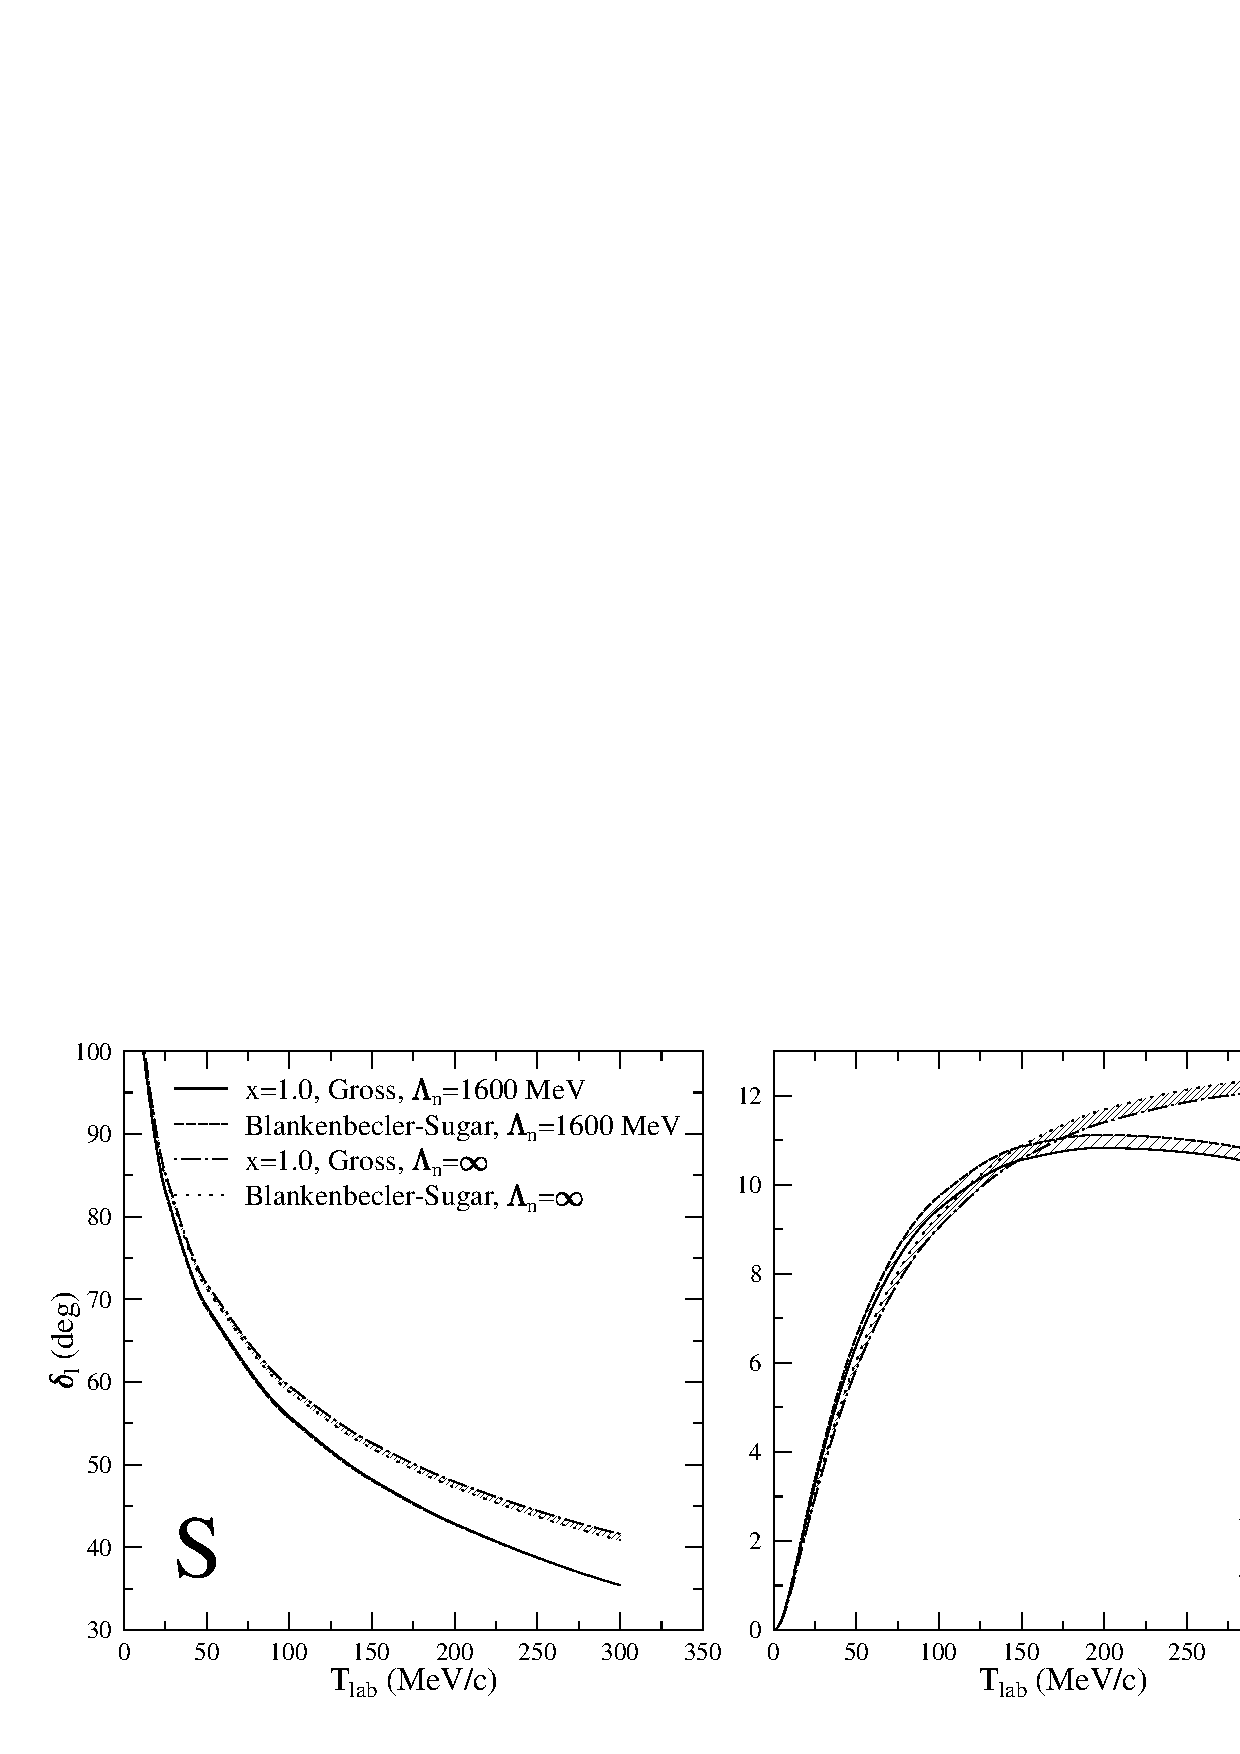
\includegraphics[width=5.5in]{graphics/phase_coup_infty.pdf}}
\caption{S- and D- wave phase shifts calculated for the various
models listed in Table I comparing results with
$\Lambda_n=1600~MeV$ (light shading) to those with
$\Lambda_n=\infty$ (dark shading). }\label{QPphasesI}
\end{figure}


Figure \ref{QPphases} shows S- and D-wave phase shifts calculated for the
various quasipotential models with $\Lambda_n=1600~MeV$. The
phase shifts for all models are within $0.5$ degrees over the range
$0 < T_{lab}<300~MeV$. This implies that there is very little model
dependence once the coupling constants are fixed to give the same binding
energy. This is in contrast with the results shown in Fig. 17 of Ref.
\cite{BrownandJ} where the coupling constant was fixed arbitrarily and
considerable
variation was seen in the phase shifts. Figure \ref{QPphasesI} shows a
comparison of the range of phase shifts calculated with $\Lambda_n=1600~MeV$
(light shading) with those with $\Lambda_n=\infty$ (small
cross-hatched band). The spread in values of the phase shifts with
$\Lambda_n=\infty$ is still small, however, a substantial sensitivity to
the cutoff mass is apparent. If phase shift data were available for this
model and included in the fit, as is the case with the NN interaction
models, the fit would tend to constrain the value of any parameter which
tended to generate substantial variation in the phase shifts.


\begin{figure}
\centerline{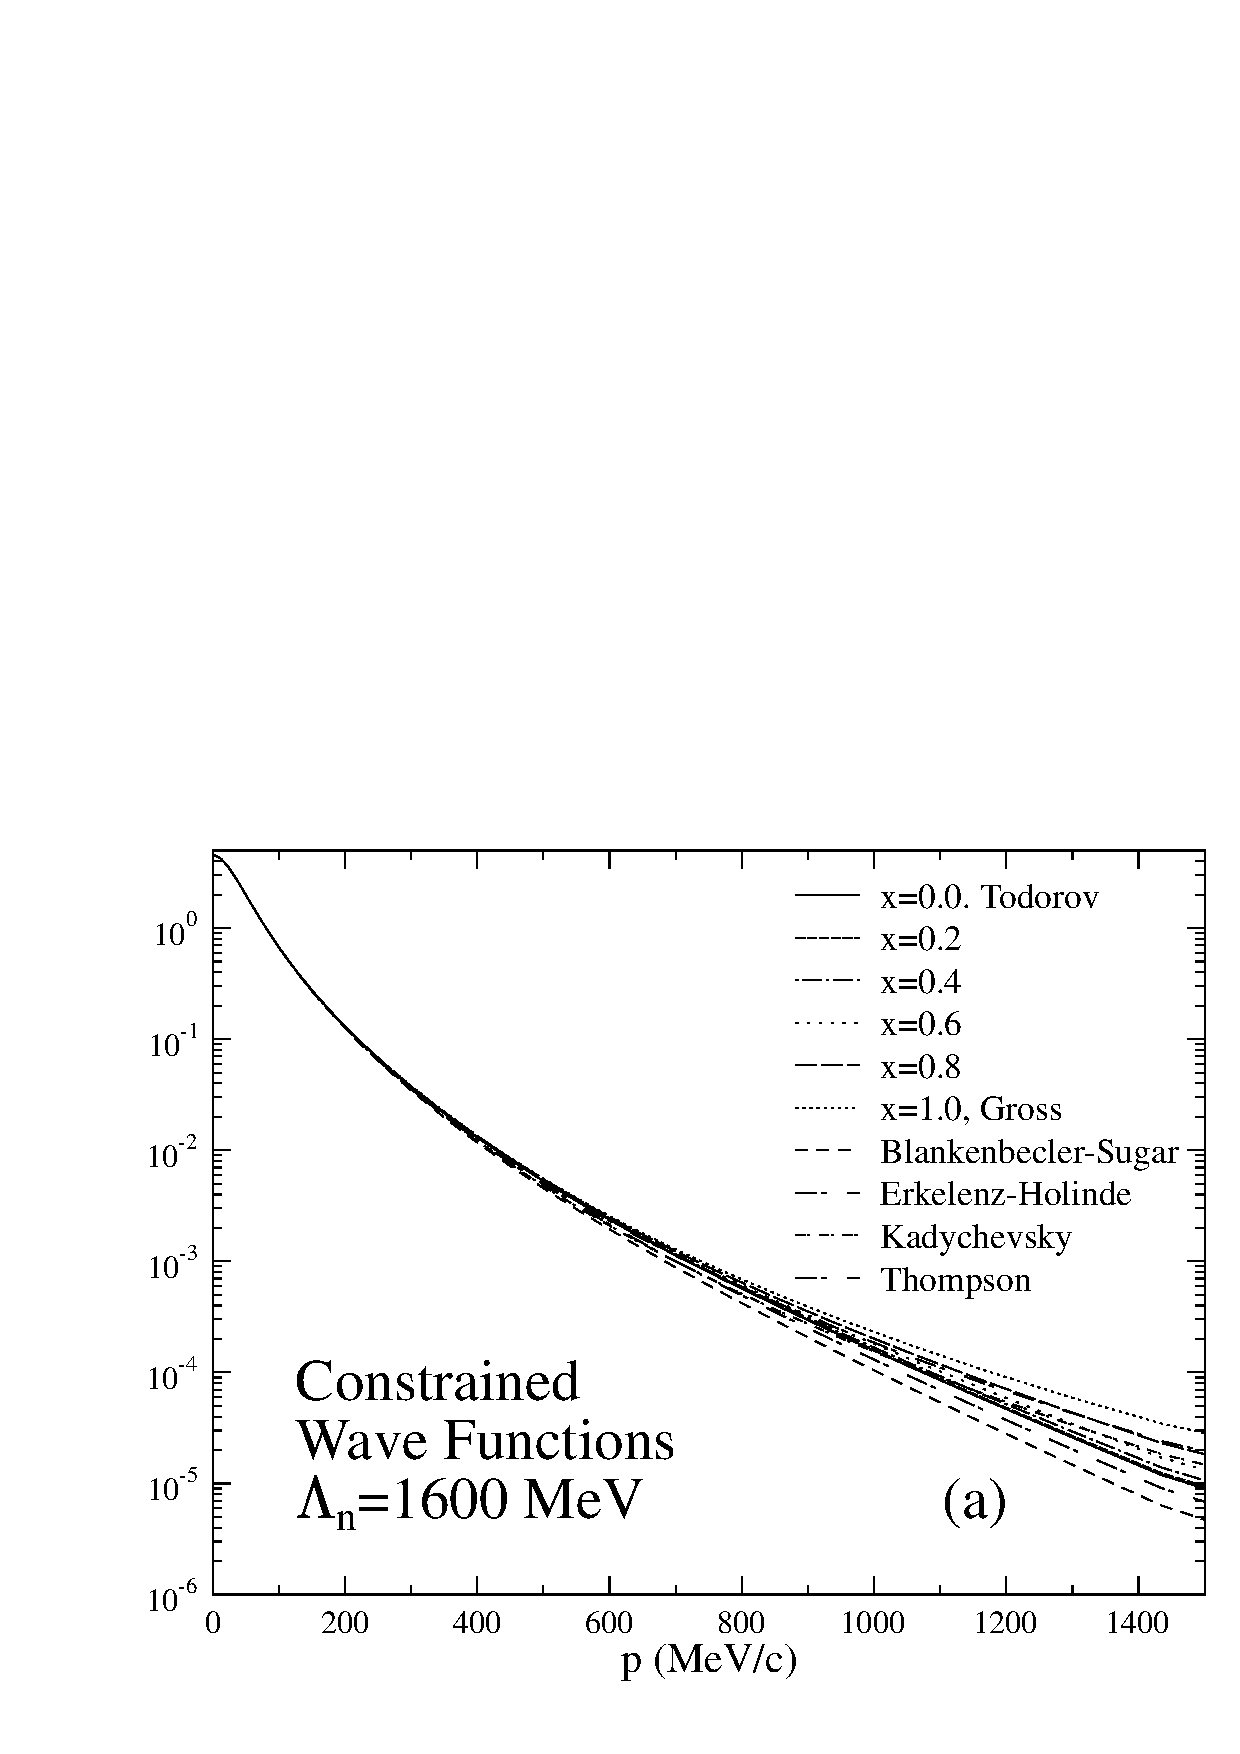
\includegraphics[width=4.5in]{graphics/wave_coup.pdf}}
\centerline{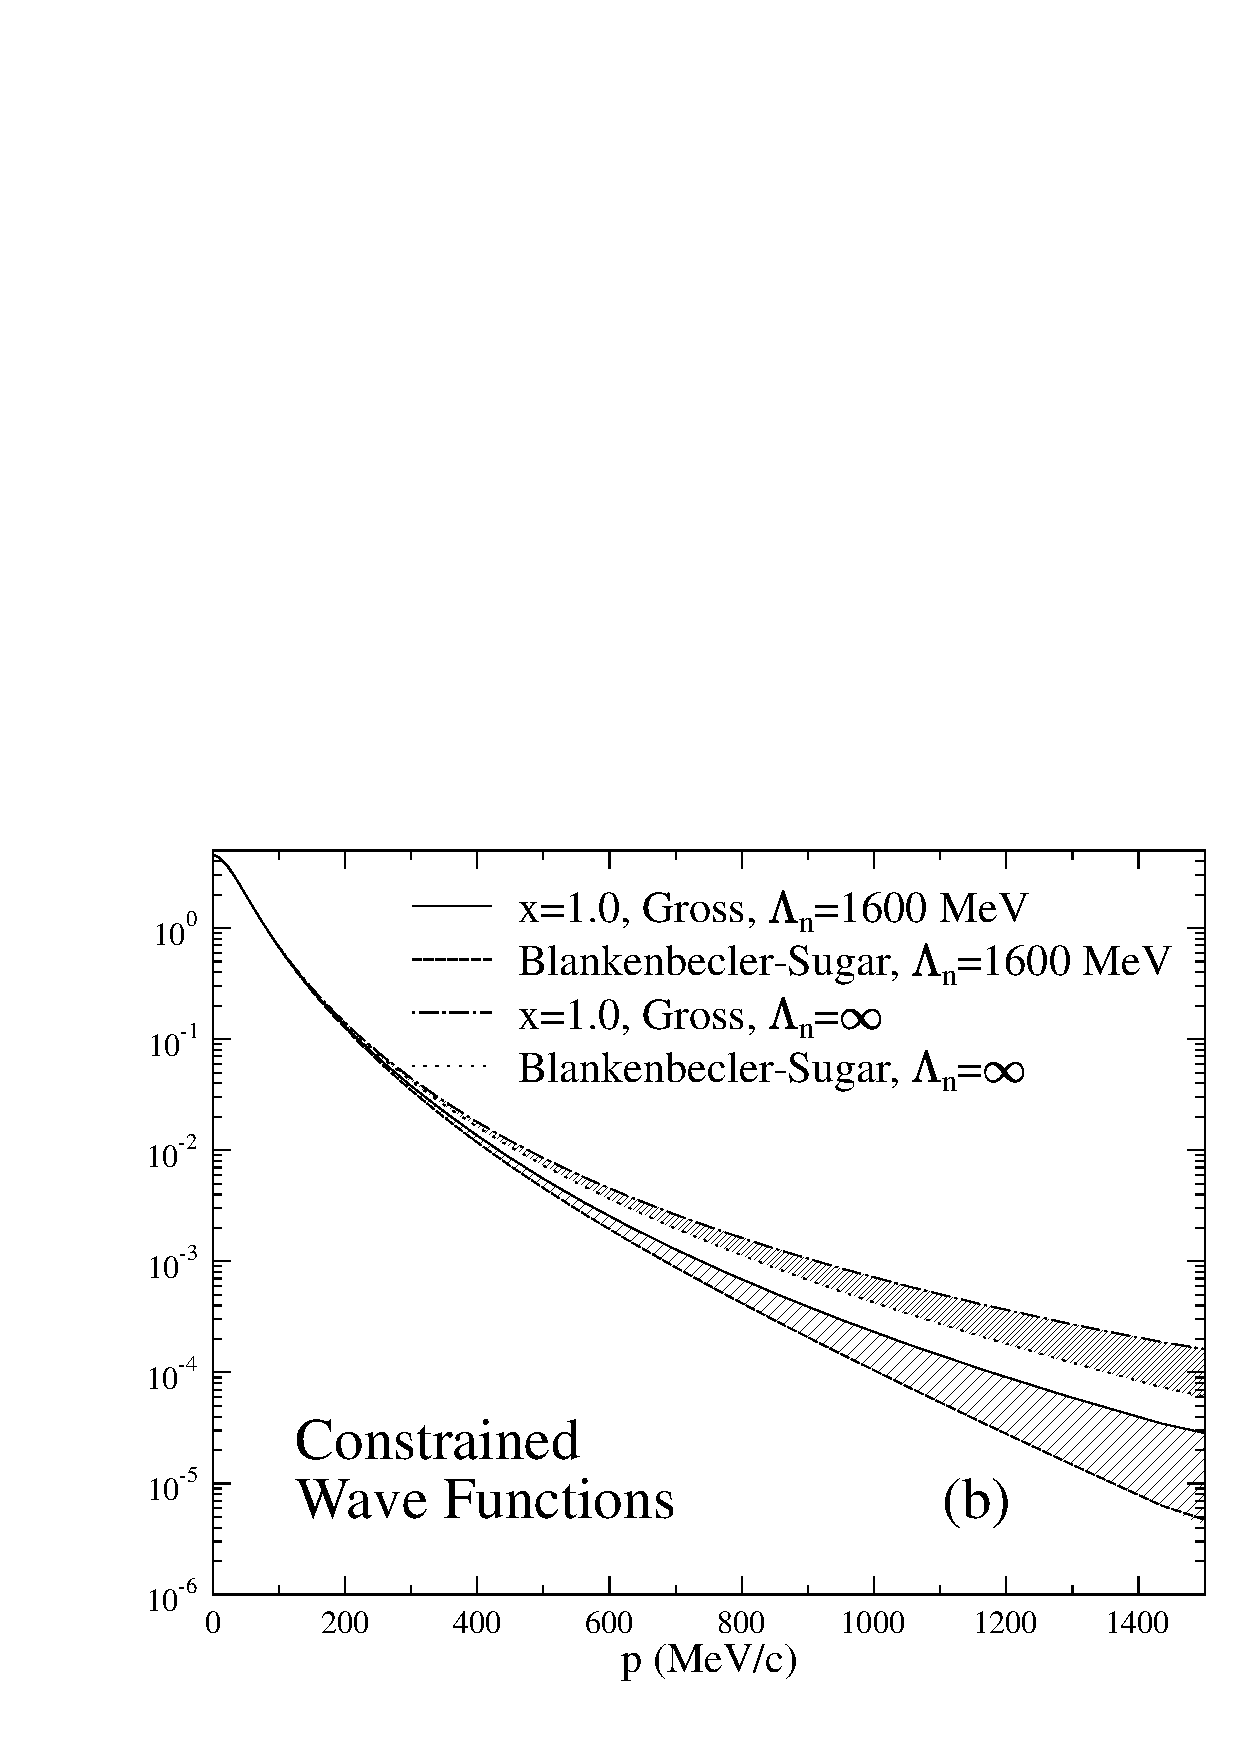
\includegraphics[width=4.5in]{graphics/wave_coup_infty.pdf}}
   \caption{Constrained quasipotential momentum space wave functions
            calculated for the
            various models listed in Table I. Figure (a) shows
            the various models with $\Lambda_n=1600~MeV$, while the
            Fig. (b) compares this range of results with that
            with $\Lambda_n=\infty$.}\label{QPwaves}
\end{figure}

Figure \ref{QPwaves} shows the constrained quasipotential momentum-space
wave functions
calculated for the various models listed in Table \ref{quasitable}. All of
the wave functions give similar values below about $200~MeV$ but tend to
diverge as the momentum increases. This is not an unexpected result since
the quasipotential propagators are very similar at low $p$ but will differ
increasingly from one another as the momentum increases. Similarly, the
effect of the nucleon cutoff will become more apparent at larger momenta.

\end{document}
